% !TEX root = report.tex

\subsection{Force calculation}
\subsubsection{\texttt{FORCLJ} subroutine}
\label{sssec:forclj}

The subroutine will first calculate the Cartesian distance between 2 atoms.
It will call \texttt{ELJ} subroutine for each pair of atoms $i$ and $j$, in which
the force between these $2$ atoms in both Cartesian and reduced coordinates
are calculated, and denoted as \texttt{fo} and \texttt{fos}, respectively.
More detailedly, \texttt{ELJ} uses the Lennard--Jones scheme.

The Lennard--Jones potential has general form
\begin{equation}
	U(r) = 4\varepsilon \bigg( \Big( \frac{ \sigma }{ r } \Big) ^ {12} -
	\Big( \frac{ \sigma }{ r } \Big) ^ 6 \bigg),
\end{equation}
where $r$ is the distance between $2$ atoms, $\sigma$ and $\varepsilon$
are constants.
The force is calculated by
\begin{equation}
	\bm{F}_{ji} = \frac{ 24\varepsilon }{ \sigma } (\bm{r}_j - \bm{r}_i)
	\bigg( 2\Big( \frac{ \sigma }{ r } \Big) ^ {14} -
	\Big( \frac{ \sigma }{ r } \Big) ^ 8 \bigg),
\end{equation}
where $r = \lvert \bm{r}_j - \bm{r}_i \rvert$, or equivalently, its scalar form
\begin{equation}
	F(r) = \frac{ 24\varepsilon }{ \sigma }
	\bigg( 2\Big( \frac{ \sigma }{ r } \Big) ^ {13} -
	\Big( \frac{ \sigma }{ r } \Big) ^ 7 \bigg),
\end{equation}
which is plotted in Fig. \ref{fig:ljar}.

\begin{figure}[h]
	\centering
	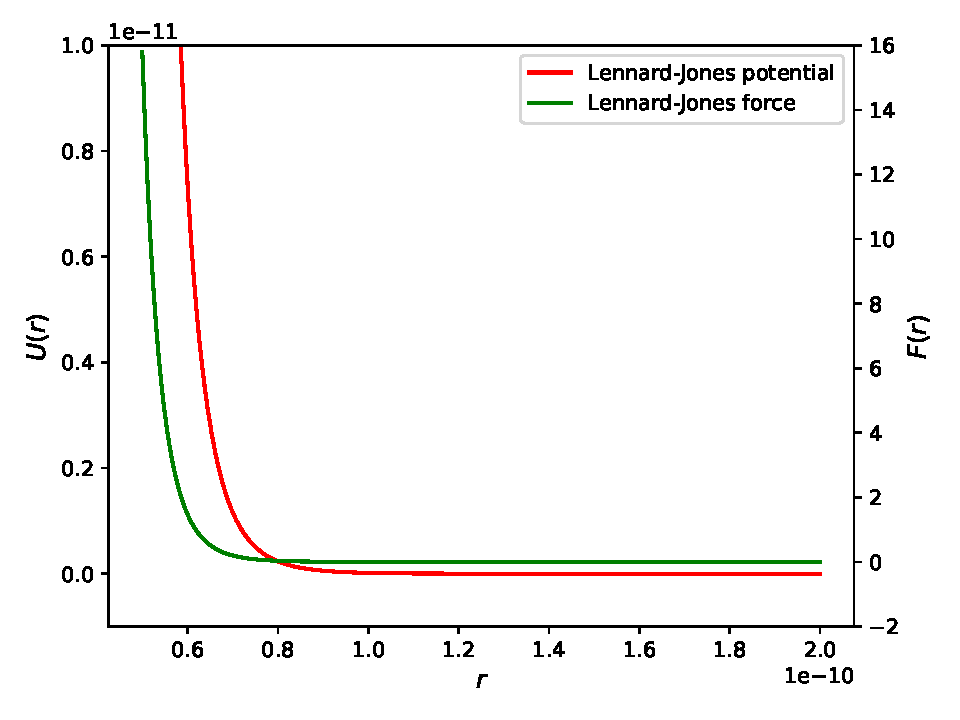
\includegraphics[width=0.5\linewidth]{lj_ar.pdf}
	\caption{Lennard--Jones potential and force for $\ce{Ar}$, as a function of
		distance between $2$ atoms, with
		$\sigma=3.405\times 10^{-10}\si{\meter}$,
		$\varepsilon = 1.654\times 10^{-21}\si{\joule}$.\cite{buffalomd}}
	\label{fig:ljar}
\end{figure}

Back to \texttt{FORCLJ} subroutine,
it considers 2 cases: particle $j$ and $i$ in the same cell and
in different cells, the first case is trivial, in the second case,
we need to add multiple times of primitive vectors and then calculate distance
$r_{ji}$, and the rest steps are the same as first case. In both cases, we do not
consider interaction out of the radius $r_{\text{cut}}$.
It appends \texttt{fo} and \texttt{fos} modified by \texttt{ELJ}
subroutine to the \texttt{f} and \texttt{fs}, respectively.


\subsubsection{\texttt{FORC} subroutine}
\label{sssec:forc}

If \texttt{FORCLJ} is used for analytical computation, then this subroutine is
used as numerical methods.
We have talked about \texttt{RDPP} subroutine before, stating that it reads
$n (n+1)$ columns of potentials and forces, denoted as \texttt{vpp} and
\texttt{fpp}, respectively.
The potentials interpolated by quadratic functions, the forces are also
calculated similar process.


\subsubsection{\texttt{UPDG} subroutine}

This part is used to update several quantities of cell during calculations.

Here \texttt{avec} is $h$, \texttt{avecd} is $\dot{ h }$, thus $g = h\tran h$
and $\dot{g}  = \dot{ h }\tran h + h \dot{ h }\tran$, \texttt{gm1} is $g^{-1}$
and \texttt{gmgd} is $g^{-1} \dot{g}$. \texttt{sigma} is the reciprocal lattice
vectors $\sigma$.

It first reads a flag \texttt{itg} to see if $\sigma$ and $V$ need to be calculated,
if it is `yes', then do the following things:
Firstly calculates $\sigma$ by the components of $h$, and then calculate the
MD cell volume by
\begin{equation}
	V = \sigma \cdot h,
\end{equation}
and then calculate $g$, $\dot{ g }$, $g^{-1}$, $g^{-1}\dot{g}$, respectively.


\subsubsection{\texttt{SIGS} and \texttt{SIGP} subroutine}
\label{sssec:sigs&p}

\texttt{SIGP} subroutine is used to calculate lattice vectors accelerations
based on `new cell dynamics', i.e., according to $\eqref{eq:rpsdd}$ and
$\eqref{eq:wenzhdd2}$; while \texttt{SIGS} is based on `strain dynamics',
i.e., $\eqref{eq:rpsdd}$ and $\eqref{eq:wenzhdd}$.
At last, the result returned is $\ddot{h}$.

In \texttt{SIGS} subroutine,
firstly calculates $f_0^{-1}$, by definition it is
\begin{equation}
	f_0^{-1} = \frac{ h_0 \tran h_0}{ V_0^2 },
\end{equation}
then set an argument \texttt{avint} to temporally store $\ddot{h}$,
and perform calculation $\ddot{h} = \ddot{h} f_0^{-1}$.
This subroutine also returns $\ddot{h}$ in the end.

In \texttt{SIGP} subroutine,
firstly calculates $f^{-1}$, by definition we know it is
\begin{equation}
	f^{-1} = \frac{ h \tran h }{ V^2 },
\end{equation}
and $e = \dot{ h }\tran \dot{ h }$, as stated above, as well as
a $3\times 3 \times 3 \times 3$ tensor
\begin{equation}
	f ' = \frac{ \partial f }{ \partial h_{ij} } = (\sigma'_{ij})\tran \sigma
	+ \sigma \tran \sigma'_{ij},
\end{equation}
where $\sigma'$ is denoted as \texttt{sigmap} in code, another $3\times 3
	\times 3 \times 3$ tensor.
$\dot{f}_0 = \dot{ \sigma } \tran \sigma + \sigma \tran \dot{ \sigma }$ is
also calculated.
$f^{-1} = \sum_{k, l} e_{lk} f'_{ijkl}$, and $\sigma^{-1} = h \dot{ f }$.
Then final returns $\ddot{h}$. As stated above, $h = (1 + \epsilon) h_0$,
where $h_0 = \{ \bm{a}_0, \bm{b}_0, \bm{c}_0 \}$.

